\documentclass[a4paper,10pt]{scrartcl}[2003/01/01]
\usepackage[ngerman]{babel}
\usepackage[T1]{fontenc}
\usepackage{inputenc}
\usepackage{graphicx}
\usepackage{listings}
\usepackage{enumerate}
\usepackage{pstricks}
\title{Software Architectures}
\subtitle{Exercise 4}
\author{ Felix Baumann \\ Manuel Gottschlich \\  Alexey Gy\"ori 352678 \\ Vincent Wehrwein \\ Markus Weller 352466}
\begin{document}
    \maketitle
    
    \section*{Aufgabe 5.1}
        \subsection*{a)}
         $$f(a,b) = abs(max(a,b))$$
        \subsection*{b)}
         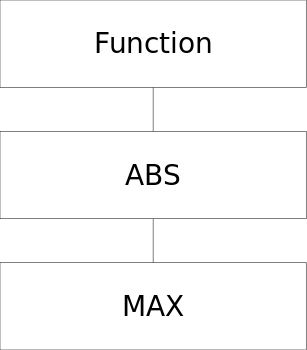
\includegraphics[scale=0.5]{dia1}
        \subsection*{c)}
        
        \subsection*{d)}
        
    \section*{Aufgabe 5.2}
        \subsection*{a)}
        \subsection*{b)}
        \subsection*{c)}
        
    \section*{Aufgabe 5.3}
    
$n!$ Combinations
   
    \section*{Aufgabe 5.4}
Software application architecture is the process of defining a structured solution that meets all of the technical and operational requirements, while optimizing common quality attributes such as performance, security, and manageability. It involves a series of decisions based on a wide range of factors, and each of these decisions can have considerable impact on the quality, performance, maintainability, and overall success of the application.

\end{document}